\chapter{The Rational Numbers}

On the integers we have the arithmetic operations of addition, subtraction, and multiplication, but we generally can't divide integers and expect the result to be another integer. Instead, we have \zcrefnamed{theorem:euclidean-division} which establishes division with remainder, and in the previous chapters we introduced the basics of the theory of integer divisibility and modulo arithmetic. Nevertheless, there is a clear sense of ratios of integers, even if such ratios are not necessarily integers. It is thus natural to introduce the concepts of \emph{integer fractions} and the \emph{rational numbers}.

\section{Integer Fractions}

\begin{definition}
  An \define{integer fraction} is an expression of the form
  \begin{equation*}
    \frac{a}{b}
  \end{equation*}
  in which $a$ is an integer and $b$ is a positive integer. In such an integer fraction, the integer $a$ is called the \define{numerator} and the positive integer $b$ is called the \define{denominator}. Furthermore:
  \begin{enumerate}
  \item An integer fraction $\frac{a}{b}$ is said to be \define{reduced} or \define{in lowest terms} if $a$ and $b$ are relatively prime.
  \item An integer $a$ can be presented as an integer fraction by $\frac{a}{1}$.
  \item An integer fraction of the form $\frac{1}{b}$ is called a \define{unit fraction}.
  \end{enumerate}
\end{definition}

While it is common to think of rational numbers as integer fractions, there is a subtle distinction between the concepts of integer fractions and rational numbers. For example, the two integer fractions $\frac{4}{3}$ and $\frac{8}{6}$ have different expressions in terms of their numerators and denominators, but we think of them as representing the \emph{same} rational number. The rational sameness relation on integer fractions is defined as follows.

\begin{definition}
  Two integer fractions $\frac{a}{b}$ and $\frac{c}{d}$ are considered the \define{same} if
  \begin{equation*}
    ad-bc=0.
  \end{equation*}
  The set $\mathbb{Q}$ of \define{rational numbers} is defined according to the following rules:
  \begin{enumerate}
  \item To construct a rational number, one has to construct an integer fraction.
  \item To prove that two rational numbers $\frac{a}{b}$ and $\frac{c}{d}$ are equal, one has to prove that $ad-bc=0$.
  \end{enumerate}
\end{definition}

\begin{figure}[t]
  \centering
  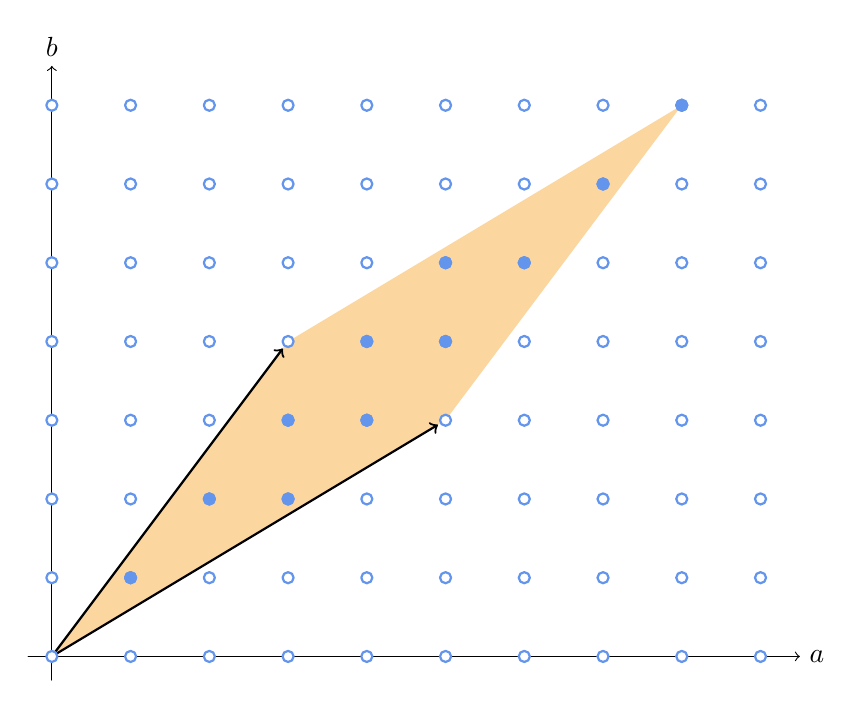
\begin{tikzpicture}[scale=1,line join=round,line cap=round]
    
    % Define primes and half-values
    \def\p{23}
    \def\q{13}

    % Draw coordinate axes
    \draw[->] (-0.3,0) -- (9.5,0) node[right] {$a$};
    \draw[->] (0,-0.3) -- (0,7.5) node[above] {$b$};

    \node[circle,minimum size=2pt,inner sep=0] (A) at (3,4) {};
    \node[circle,minimum size=2pt,inner sep=0] (B) at (5,3) {};

    \fill[YellowOrange,opacity=.4] (0,0) -- (3,4) -- (8,7) -- (5,3) -- cycle;
    
    \draw[->,thick,shorten >=2pt] (0,0) -- (A);
    \draw[->,thick,shorten >=2pt] (0,0) -- (B);
    
    \foreach \x in {0,1,2,3,4,5,6,7,8,9} {
      \foreach \y in {0,1,2,3,4,5,6,7} {
        \draw[CornflowerBlue,fill=white,thick] (\x,\y) circle (2pt);
      }
    }

    \draw[CornflowerBlue,fill,thick] (1,1) circle (2pt);
    \draw[CornflowerBlue,fill,thick] (2,2) circle (2pt);    
    \draw[CornflowerBlue,fill,thick] (3,3) circle (2pt);
    \draw[CornflowerBlue,fill,thick] (4,4) circle (2pt);
    \draw[CornflowerBlue,fill,thick] (5,5) circle (2pt);
    \draw[CornflowerBlue,fill,thick] (3,2) circle (2pt);
    \draw[CornflowerBlue,fill,thick] (4,3) circle (2pt);
    \draw[CornflowerBlue,fill,thick] (5,4) circle (2pt);
    \draw[CornflowerBlue,fill,thick] (6,5) circle (2pt);
    \draw[CornflowerBlue,fill,thick] (7,6) circle (2pt);
    \draw[CornflowerBlue,fill,thick] (8,7) circle (2pt);

  \end{tikzpicture}
  \caption[Lattice points in a parallelogram]{There are 11 lattice points in the parallelogram spanned by $(3,4)$ and $(5,3)$, not including the points $(0,0)$, $(3,4)$, and $(5,3)$. This number is equal to the quantity $4\cdot 5-3\cdot 3$, and it is also equal to the number of reduced integer fractions between $\frac{3}{4}$ and $\frac{5}{3}$ with denominators not exceeding $7$.}
  \label{figure:lattice-points-parallelogram}
\end{figure}

\begin{remark}
More generally, the quantity $\abs{bc-ad}$ is a measure for how far apart the fractions $\otfrac{a}{b}$ and $\otfrac{c}{d}$ are. Assuming that the inequality $\otfrac{a}{b}\leq \otfrac{c}{d}$ holds so that $bc-ad\geq 0$, we will show in \zcref{theorem:meaning-explanation-determinant-fractions} that the number
\begin{equation*}
  bc-ad
\end{equation*}
counts the number of fractions $\otfrac{a}{b}<\otfrac{s}{t}<\otfrac{c}{d}$ such that the denominator $t$ does not exceed $b+d$. Indeed, if $\otfrac{a}{b}=\otfrac{c}{d}$ then there should be no fractions strictly between $\otfrac{a}{b}$ and $\otfrac{c}{d}$, as is signified by the number $bc-ad=0$.

The quantity $k=\abs{bc-ad}$ is also the area of the parallelogram spanned by $(a,b)$ and $(c,d)$. Moreover, there are exactly $k$ lattice points in this parallelogram, excluding multiples of $(a,b)$ and $(c,d)$.
\end{remark}

\begin{theorem}
  For any integer fraction $\frac{a}{b}$ there is a unique reduced integer fraction $\frac{c}{d}$ such that $\frac{a}{b}\sim\frac{c}{d}$. Consequently, two integer fractions are the same if and only if they have the same reduced integer fraction.
\end{theorem}

\begin{proof}
  The reduced integer fraction $\frac{a'}{b'}$ associated to an integer fraction $\frac{a}{b}$ is defined by the integers
  \begin{equation*}
    a':=\frac{a}{\gcd(a,b)}\qquad\text{and}\qquad b':=\frac{b}{\gcd(a,b)}.
  \end{equation*}
  This definition makes sense within the integers, since $a$ and $b$ are both divisible by the greatest common divisor $\gcd(a,b)$. To see that the fractions $\frac{a}{b}$ and $\frac{a'}{b'}$ are the same, we compute
  \begin{equation*}
    ab'-ba'=a\frac{b}{\gcd(a,b)}-b\frac{a}{\gcd{a,b}}=0.
  \end{equation*}
  This shows that for every integer fraction is the same to at least one reduced integer fraction. For the uniqueness claim, we will show that any two reduced integer fractions that are the same, have the same numerator and denominator. Let $\frac{a}{b}$ and $\frac{c}{d}$ be two reduced integer fractions such that
  \begin{equation*}
    ad-bc=0,
  \end{equation*}
  so that the equation $ad=bc$ holds. Then we have $d\mid bc$, from which it follows that $d\mid b$ by \zcref{proposition:coprime-divides-product}. Conversely, we have $b\mid ad$ so that $b\mid d$. Since $b$ and $d$ are positive integers mutually dividing each other, it follows that $b=d$. Consequently, we obtain that $ab=bc$, which gives that $a=c$.
\end{proof}

By the remarks preceeding the previous theorem, we should expect there to be exactly one reduced integer fraction in the interval strictly between $\frac{a}{b}$ and $\frac{c}{d}$, provided that
\begin{equation*}
  bc-ad=1.
\end{equation*}
This is the content of the following theorem.

\begin{theorem}
  Suppose that $\frac{a}{b}$ and $\frac{c}{d}$ are reduced integer fractions satisfying
  \begin{equation*}
    bc-ad=1.
  \end{equation*}
  Then there is exactly one reduced integer fraction $\frac{a}{b}<\frac{s}{t}<\frac{c}{d}$, namely the \define{mediant}
  \begin{equation*}
    \frac{a+c}{b+d}.
  \end{equation*}
\end{theorem}

\begin{proof}
  First, we claim that the function
  \begin{equation*}
    t\mapsto \frac{a+tc}{b+td}
  \end{equation*}
  defines a bijection from the positive reduced integer fractions to the reduced integer fractions in the interval of integer fractions strictly between $\frac{a}{b}$ and $\frac{c}{d}$. Indeed, if $\frac{p}{q}$ is a positive reduced integer fraction, then its value under this map is
  \begin{equation*}
    \frac{qa+pc}{qb+pd}.
  \end{equation*}
\end{proof}

\begin{definition}
  Integer fractions can be added, subtracted, and multiplied according to the following rules:
  \begin{equation*}
     \frac{a}{b}+\frac{c}{d} = \frac{ad+bc}{bd}, \qquad \frac{a}{b}-\frac{c}{d} = \frac{ad-bc}{bd}, \qquad\text{and}\qquad \frac{a}{b}\frac{c}{d} = \frac{ac}{bd}.
  \end{equation*}
  Furthermore, if the numerator of $\frac{a}{b}$ is nonzero, then we can invert $\frac{a}{b}$ by:
  \begin{equation*}
    \left(\frac{a}{b}\right)^{-1} = \frac{b}{a}.
  \end{equation*}
\end{definition}

\begin{theorem}
  Addition, subtraction, multiplication and inversion of integer fractions satisfies the axioms of a field:
  \begin{align*}
    (x+y)+z & = x + y+ z & (xy)z & = x(yz) \\
    x+y & = y+x & xy &= yx \\
    0+x & = x & 1x & = x \\
    x-x & = 0 & xx^{-1} & = 1 \\
    & & x(y+z) & = xy+xz.
  \end{align*}
  Furthermore, adding, subtracting, multiplying or inverting integer fractions preserves the sameness relation on integer fraction, in the sense that if we substitute each integer fraction in a sum, difference, product, or inversion by one that is the same to the original, the result will be the same.
\end{theorem}

\section{The Irrationality of Square Roots}

\begin{theorem}\label{theorem:irrational-sqrt}
  If a natural number $n$ is not a perfect square, then its square root $\sqrt{n}$ is irrational.
\end{theorem}

\begin{proof}
  We will prove the theorem by deriving a contradiction under the assumption that there is a reduced integer fraction $\frac{a}{b}$ such that
  \begin{equation*}
    \frac{a^2}{b^2}=n.
  \end{equation*}
  This equation is equivalent to the equation $a^2=nb^2$. Furthermore, we may assume without loss of generality that $a$ and $b$ are relatively prime, because we can always divide both sides of the equation $a^2=n b^2$ by $\gcd(a,b)^2$. By this very equation, it follows that $b^2\mid a^2$. Thus we have
  \begin{equation*}
    b^2=\gcd(a^2,b^2)=\gcd(a,b)^2=1,
  \end{equation*}
  and we see that $b=1$. However, this implies that $n=a^2$ is a perfect square, contradicting our assumtion that $n$ is not a perfect square.
\end{proof}

\section{Continued Fractions}

Consider the numbers $a=193$ and $b=71$. Running Euclid's algorithm on these numbers to find their greatest common divisor, we obtain:
\begin{align*}
  193 & = 2\cdot 71 + 51, \\
  71 & = 1\cdot 51 + 20, \\
  51 & = 2\cdot 20 + 11, \\
  20 & = 1\cdot 11 + 9, \\
  11 & = 1\cdot 9 + 2, \\
  9 & = 4\cdot 2 + 1, \\
  2 & = 2\cdot 1 + 0.
\end{align*}
If we divide the top equation through by $71$, we obtain the equation
\begin{equation*}
  \frac{193}{71}=2+\frac{51}{71}.
\end{equation*}
Similarly, we have $\frac{71}{51}=1+\frac{20}{51}$, and so on. Rewriting $\frac{51}{71}$ to the fraction $\otfrac{1}{\frac{71}{51}}$ then allows us to obtain:
\begin{equation*}
  \frac{193}{71}=2+\frac{1}{1+\frac{20}{51}}.
\end{equation*}
Continuing this way, we find that
\begin{equation*}
  \frac{193}{71}=2+\cfrac{1}{1+\cfrac{1}{2+\cfrac{1}{1+\cfrac{1}{1+\cfrac{1}{4+\tfrac{1}{2}}}}}}.
\end{equation*}
Such iterated fractions are called \define{continued fractions}. The fraction $\frac{193}{71}$ is a famously accurate approximation of Euler's number $e$, being correct to within a distance of $\otfrac{1}{71^2}$, and its continued fraction is the start of the continued fraction expansion of $e$. As we just saw, continued fractions are closely related to Euclid's algorithm, and indeed they are used for rational approximations of real numbers.

\begin{definition}
  A \define{finite (simple) continued fraction} is an expression of the form
  \begin{equation*}
    q_0+\cfrac{1}{q_1+\cfrac{1}{q_2+\cfrac{1}{\cdots + \cfrac{1}{q_n}}}},
  \end{equation*}
  where $q_0$ is an arbitrary integer, each $q_i$ with $i>0$ is a positive integer, and furthermore $q_n>1$. The adjective \emph{simple} refers to the fact that only the number $1$ is ever used as a numerator. We will generally assume that continued fractions are simple, so we will omit this disambiguation. A commonly used compact notation for finite simple continued fractions is $[q_0,q_1,q_2,\ldots,q_n]$.

  Infinite continued fractions are infinite expressions of the form
  \begin{equation*}
    q_0+\cfrac{1}{q_1+\cfrac{1}{q_2+\cfrac{1}{\cdots}}}.
  \end{equation*}
  A more compact notation for infinite continued fractions is $[q_0,q_1,\ldots]$. The numbers $q_i$ in a continued fraction $[q_0,q_1,\ldots]$ are called the \define{partial quotients}.
\end{definition}

Carl Friedrich Gauss had the following elegant notation for continued fractions, which is not widely used anymore:
\begin{equation*}
  q_0+\mathop{\mathrm{K}}\limits_{i=1}^{\infty} \frac{1}{q_i} =
  q_0+\cfrac{1}{q_1+\cfrac{1}{q_2+\cfrac{1}{\cdots}}}.
\end{equation*}
Here, the letter K stands for \emph{Kettenbruch}, the German word for continued fraction. In the present chapter we will mostly focus our attention on finite continued fractions. Infinite continued fractions are an important way of uniquely representing arbitrary real numbers, and they have applications in Pells equations, or more generally the study of quadratic fields, the theory of Diophantine approximations, and the theorems establishing the transcendence of numbers like $\pi$ and $e$.

\begin{theorem}
  Every reduced integer fraction can be uniquely represented as a finite continued fraction.
\end{theorem}

\begin{proof}
  Consider two relatively prime integers $a$ and $b$ with $b>0$. The proof is by strong induction on $b$. In the base case, where $b=1$, the unique finite continued fraction representing $\frac{a}{b}$ is the continued fraction $[a]$, which has no fractional part. 

  By \zcrefnamed{theorem:euclidean-division} there is a uniqe pair $(q,r)$ of integers with $0\leq r<b$ such that $a=qb+r$. In the case where $r=0$, we obtain that $\frac{a}{b}=q$, from which it follows that $[q]$ is the unique finite continued fraction representing $\frac{a}{b}$. In case $r>0$ we write
  \begin{equation*}
    \frac{a}{b} = q + \cfrac{1}{\frac{b}{r}}.
  \end{equation*}
  The integers $b$ and $r$ are relatively prime with $r<b$. By the strong induction hypothesis, it follows that $\frac{b}{r}$ is uniquely represented as a continued fraction $[q_1,q_2,\ldots,q_n]$. It follows that $[q,q_1,\ldots,q_n]$ is a continued fraction representing $\frac{a}{b}$. Furthermore, it is the unique such representation, since the integer part of a continued fraction is uniquely determined as the largest integer below $\frac{a}{b}$.
\end{proof}

\begin{definition}
  Consider a continued fraction $[q_0,\ldots,q_n]$ or $[q_0,q_1,\ldots]$. The continued fractions
  \begin{equation*}
    \frac{a_i}{b_i}:=[q_0,\ldots,q_i]
  \end{equation*}
  are called the \define{convergents} of the continued fraction.
\end{definition}

The first few convergents of a continued fraction $[q_0,q_1,\ldots]$ are
\begin{equation*}
  \frac{a_0}{b_0} = \frac{q_0}{1},\qquad
  \frac{a_1}{b_1} = \frac{q_0q_1+1}{q_1},\qquad
  \frac{a_2}{b_2} = \frac{q_0q_1q_2+q_0+q_2}{q_1q_2+1},\qquad
  \ldots
\end{equation*}
so that $a_0=q_0$, $b_0=1$, $a_1=q_0q_1+1$, $b_1=q_1$, and so on.
For example, consider the continued fraction $[2,1,2,1,1,4,2]$, which we used at the beginning of this section to motivate the definition of continued fractions. Its convergents are:
\begin{equation*}
  \frac{a_0}{b_0}=\frac{2}{1},\quad
  \frac{a_1}{b_1}=\frac{3}{1},\quad
  \frac{a_2}{b_2}=\frac{8}{3},\quad
  \frac{a_3}{b_3}=\frac{11}{4},\quad
  \frac{a_4}{b_4}=\frac{19}{7},
  \ldots
\end{equation*}
This sequence of fractions provides increasingly better rational approximations of Euler's number $e$. Notice that the numerators and denominators are increasing. In fact, one can check that the fraction $\frac{19}{7}$ is the best approximation of $e$ using a denominator not exceeding $7$, and the distance from $\frac{19}{7}$ to $e$ does not exceed $\frac{1}{7^2}$.

We are thus naturally led to the question of determining the value of a finite continued fraction $[q_0,\ldots,q_n,x]$, provided that we know the previous values. Note that the variable $x$ occurs deeply nested in the continued fraction. At first sight, computing the value for $[q_0,\ldots,q_n,x]$ thus seems increasingly complicated as $n$ gets larger. Euler faced the same problem in 1744, and he discovered a nice pattern \cite[art.~7]{euler1744}. He recognized that if we recursively define the sequences $a_n$ and $b_n$ by
\begin{align*}
  a_0 & := q_0, & a_1 & := q_1q_0 + 1, & a_{n+2} & := q_{n+2}a_{n+1}+a_n, \\
  b_0 & := 1, & b_1 & := q_1, & b_{n+2} & := q_{n+2}b_{n+1}+b_n,
\end{align*}
then the fraction $\frac{a_n}{b_n}$ is the $n$\supth{} convergent of the continued fration $[q_0,q_1,\ldots]$. This observation works even if the partial quotients $q_i$ aren't integers, which Euler took advantage of in order to express some functions as continued fractions.

A key ingredient of Euler's inductive proof is the identity
\begin{equation*}
  [q_0,\ldots,q_n,r]=[q_0,\ldots,q_n+\tfrac{1}{r}].
\end{equation*}
Thus, we will need to distinguish in notation for the numerators and denominators of different continued fractions with the same value. A good way to do this, is to explicity use the list of numbers $q_0,\ldots,q_n$ in our notation for the numerator and denominator of $[q_0,\ldots,q_n]$: They will be denoted by
\begin{equation*}
  a_{q_0,\ldots,q_n}\qquad\text{and}\qquad b_{q_0,\ldots,q_n}.
\end{equation*}
Or, to establish a more compact notation, if we write $\symbf{q}=q_0,\ldots,q_n$, then we can write $a_{\symbf{q}}$ and $b_{\symbf{q}}$ for the numerator and denominator of the continued fraction $[\symbf{q}]=[q_0,\ldots,q_n]$.

\begin{theorem}[Recurrence Theorem for Convergents]\label{theorem:recurrence-theorem-convergents}
  Define the numbers $a_{\symbf{q}}$ and $b_{\symbf{q}}$ for every finite continued fraction $[\symbf{q}]:=[q_0,\ldots,q_n]$ by list recursion as follows:
  \begin{align*}
    a_q & := q & a_{q,r} & := rq + 1, & a_{\symbf{q},r,s} & := sa_{\symbf{q},r}+a_{\symbf{q}}, \\
    b_{q} & := 1 & b_{q,r} & := r, & b_{\symbf{q},r,s} & := sb_{\symbf{q},r}+b_{\symbf{q}}.
  \end{align*}
  Then we have $\frac{a_{\symbf{q}}}{b_{\symbf{q}}}=[\symbf{q}]$.
\end{theorem}

\begin{proof}
  Since the numbers $a_{\symbf{q}}$ and $b_{\symbf{q}}$ are defined by list recursion, we will prove the claim with list induction. Note that $a_q=q$ and $b_q=1$, so that
  \begin{equation*}
    \frac{a_q}{b_q}=[q].
  \end{equation*}
  Similarly, we have $a_{q,r}=rq+1$ and $b_{q,r}=r$, so that
  \begin{equation*}
    \frac{a_{q,r}}{b_{q,r}}=\frac{rq+1}{r}=q+\frac{1}{r}=[q,r].
  \end{equation*}
  We will do one more base case. Note that $a_{q,r,s}=srq+q+s$ and $b_{q,r,s}=sr+1$. Then we have that
  \begin{equation*}
    \frac{a_{q,r,s}}{b_{q,r,s}}=\frac{srq+q+s}{sr+1}=q+\frac{s}{sr+1}=q+\cfrac{1}{r+\tfrac{1}{s}}=[q,r,s].
  \end{equation*}
  For the inductive step, consider an arbitrary list $[\symbf{q}]=[q_0,\ldots,q_n]$ and three more numbers $r$, $s$, and $t$. Using the recursive definition of $a$ and $b$ as well as the inductive hypothesis in the final equality, we note that
  \begin{equation*}
    \frac{a_{\symbf{q},r,s,t}}{b_{\symbf{q},r,s,t}}=
    \frac{ta_{\symbf{q},r,s}+a_{\symbf{q},r}}{tb_{\symbf{q},r,s}+b_{\symbf{q},r}} =
    \frac{a_{\symbf{q},r,s}+\frac{a_{\symbf{q},r}}{t}}{b_{\symbf{q},r,s}+\frac{b_{\symbf{q},r}}{t}} =
    \frac{(s+\frac{1}{t})a_{\symbf{q},r}+a_{\symbf{q}}}{(s+\frac{1}{t})b_{\symbf{q},r}+b_{\symbf{q}}} =
    \frac{a_{\symbf{q},r,s+\frac{1}{t}}}{b_{\symbf{q},r,s+\frac{1}{t}}} =
    [\symbf{q},r,s+\tfrac{1}{t}].
  \end{equation*}
  This completes the proof, since $[\symbf{q},r,s+\tfrac{1}{t}] = [\symbf{q},r,s,t]$.
\end{proof}

\begin{theorem}[Determinant Identity for Convergents]\label{theorem:determinant-formula-convergents}
  For any continued fraction $[\symbf{q},r]=[q_0,\ldots,q_n,r]$ of length $n+2$, we have
  \begin{equation*}
    a_{\symbf{q},r}b_{\symbf{q}}-b_{\symbf{q},r}a_{\symbf{q}}=(-1)^n.
  \end{equation*}
\end{theorem}

\begin{proof}
  In the base case we have
  \begin{equation*}
    a_{q,r}b_q-b_{q,r}a_q=(rq+1)-rq=1.
  \end{equation*}
  For the inductive step, assume that $a_{\symbf{q},r}b_{\symbf{q}}-b_{\symbf{q},r}a_{\symbf{q}}=(-1)^n$. Then we compute:
  \begin{align*}
    a_{\symbf{q},r,s}b_{\symbf{q},r}-b_{\symbf{q},r,s}a_{\symbf{q},r} & = (sa_{\symbf{q},r}+a_{\symbf{q}})b_{\symbf{q},r}-(sb_{\symbf{q},r}+b_{\symbf{q}})a_{\symbf{q},r} \\
                                                                          & = a_{\symbf{q}}b_{\symbf{q},r}-b_{\symbf{q}}a_{\symbf{q},r} \\
    & = -(-1)^n.\qedhere
  \end{align*}
\end{proof}

\begin{theorem}\label{theorem:lowest-terms-convergents}
  Consider a continued fraction $[\symbf{q}]=[q_0,\ldots,q_n]$ with integer partial quotients $q_i$. Then the convergent
  \begin{equation*}
    \frac{a_{\symbf{q}}}{b_{\symbf{q}}}=[\symbf{q}]
  \end{equation*}
  is an integer fraction in lowest terms.
\end{theorem}

\begin{proof}
  If each $q_i$ is an integer, then $a_{\symbf{q}}$ and $b_{\symbf{q}}$ are determined by recursively adding and multiplying integers, so they are integers. Furthermore, the determinant identity
  \begin{equation*}
    a_{\symbf{q},r}b_{\symbf{q}}-b_{\symbf{q},r}a_{\symbf{q}}=(-1)^n.
  \end{equation*}
  shows that $\gcd(a_{\symbf{q}},b_{\symbf{q}})\mid (-1)^n$, so $a_{\symbf{q}}$ and $b_{\symbf{q}}$ are relatively prime.
\end{proof}

We summarize the above results for infinite continued fractions.

\begin{corollary}
  Consider an infinite continued fraction $[q_0,q_1,\ldots]$ and define the sequences $a_n$ and $b_n$ recursively by
  \begin{align*}
    a_0 & := q_0, & a_1 & := q_1q_0+1, & a_{n+2} & := q_{n+2}a_{n+1}+a_n, \\
    b_0 & := 1, & b_1 & := q_1, & b_{n+2} & := q_{n+2}b_{n+1}+b_n.
  \end{align*}
  Then the fraction $\frac{a_n}{b_n}$ is the $n$\supth{} convergent of $[q_0,q_1,\ldots]$, it is in lowest terms for every $n$, and we have $a_{n+1}b_n-b_{n+1}a_n=(-1)^{n}$.

  Furthermore, the numerators $a_n$ and denominators $b_n$ of the convergents of an infinite continued fraction form strictly increasing sequences of integers for $n>0$, and
  \begin{equation*}
    \frac{a_{n+1}}{b_{n+1}}-\frac{a_n}{b_n}=\frac{(-1)^n}{b_nb_{n+1}}.
  \end{equation*}
\end{corollary}

\begin{example}
  Consider, for example, the continued fraction $\varphi:=[1,1,\ldots]$ in which each partial quotient is $1$. Then the numerators and denominators of the convergents are determined recursively by
  \begin{align*}
    a_0 & := 1, & a_1 & := 2, & a_{n+2} & := a_{n+1}+a_n, \\
    b_0 & := 1, & b_1 & := 1, & b_{n+2} & := b_{n+1}+b_n.
  \end{align*}
  In other words, $a_n=F_{n+2}$ is the $(n+2)$\supnd{} Fibonacci number and $b_n=F_{n+1}$ is the $(n+1)$\supst{} Fibonacci number. The recurrence theorem furthermore implies that the Fibonacci numbers satisfy the identity
  \begin{equation*}
    F_{n+2}F_{n}-F_{n+1}F_{n+1}=(-1)^{n+1}.
  \end{equation*}
  This identity is known as \emph{Cassini's identity}.

  Furthermore, we can compute the exact value of the continued fraction $\varphi:=[1,1,\ldots]$. Notice that
  \begin{equation*}
    \varphi=[1,1,\ldots]=1+\frac{1}{[1,1,\ldots]}=1+\frac{1}{\varphi}.
  \end{equation*}
  By rewriting this equation, we see that $\varphi^2=\varphi +1$. The quadratic forumal now gives us that
  \begin{equation*}
    \varphi = \frac{1+\sqrt{5}}{2}. 
  \end{equation*}
  This number is known as the \define{golden ratio}. The continued fraction $[1,1,\ldots]$ shows that the convergents
  \begin{equation*}
    \frac{F_{n+1}}{F_n}
  \end{equation*}
  determine increasingly accurate approximations of the golden ratio.
\end{example}

\section{Farey's Series of Fractions}

The geologist John Farey Sr.~observed in a letter to the British periodical \emph{The Philosophical Magazine and Journal} \cite{farey1816} that for any three consecutive fractions $\frac{a}{b}$, $\frac{s}{t}$, and $\frac{c}{d}$ in the series $\mathcal{F}_n$, we must have
\begin{equation*}
  \frac{s}{t}=\frac{a+c}{b+d}.
\end{equation*}

\begin{definition}
  The \define{mediant} of two reduced integer fractions $\frac{a}{b}$ and $\frac{c}{d}$ is the integer fraction
  \begin{equation*}
    \frac{a}{b}\mediant\frac{c}{d} := \frac{a+c}{b+d}.
  \end{equation*}
\end{definition}

We stress that this definition of the mediant makes essential use of the assumption that the input integer fractions are in reduced form. If not, the value of the mediant could be skewed by common factors.

We can think of the mediant of two reduced integer fractions as the \emph{weighted average}, where the weights are assigned according to the ratio of their denominators:
\begin{equation*}
  \frac{a}{b}\mediant\frac{c}{d} = \frac{b}{b+d}\frac{a}{b}+\frac{d}{b+d}\frac{c}{d}.
\end{equation*}

\begin{proposition}
  The mediant satisfies the following laws:
  \begin{align*}
    x\mediant y & = y\mediant x, \\
    x\mediant x & = x, \\
    \lambda x\mediant \lambda y & = \lambda(x\mediant y).
  \end{align*}
  Furthermore, we have
  \begin{equation*}
    x\leq x\mediant y\leq y\qquad\text{and}\qquad x< x\mediant y<y
  \end{equation*}
  if $x\leq y$ or $x<y$, respectively. However, the mediant is nonunital and nonassociative, meaning that there does not exist an element $e$ such that $x\mediant e=x$ and there are integer fractions $x$, $y$, and $z$ such that $(x\mediant y)\mediant z=x\mediant(y\mediant z)$.
\end{proposition}

\begin{proof}
  To prove the interchange law, consider the integer fractions $\frac{a}{b}$, $\frac{c}{d}$, $\frac{e}{f}$, and $\frac{g}{h}$. Then we calculate
  \begin{align*}
    \left(\frac{a}{b}\mediant\frac{c}{d}\right)\mediant\left(\frac{e}{f}\mediant\frac{g}{h}\right) & = \frac{a+c}{b+d}\mediant\frac{e+g}{f+h} \qedhere
  \end{align*}
\end{proof}

\begin{theorem}
  Consider two reduced fractions $\frac{a}{b}<\frac{c}{d}$ such that
  \begin{equation*}
    bc-ad=1.
  \end{equation*}
  Then there is a unique Farey fraction of order $b+d$ strictly between $\frac{a}{b}$ and $\frac{c}{d}$: the mediant
  \begin{equation*}
    \frac{a+b}{c+d}.
  \end{equation*}
\end{theorem}

\begin{theorem}\label{theorem:meaning-explanation-determinant-fractions}
  Consider two reduced fractions $\frac{a}{b}<\frac{c}{d}$ and set
  \begin{equation*}
    k:=bc-ad.
  \end{equation*}
  Then there are exactly $k$ Farey fractions of order $\leq b+d$ strictly between $\frac{a}{b}$ and $\frac{c}{d}$.
\end{theorem}

\section{A Structural Definition of the Rational Numbers}

\begin{figure}[t]
  \centering
  \begin{tikzpicture}[every node/.style={font=\fontsize{9pt}{9pt}}]
    \node[draw,thick,circle,inner sep=1.8pt] (N01) at (0,-1) {$\dfrac{0}{1}$};
    \node[draw,thick,circle,inner sep=1.8pt] (N11) at (12,-1) {$\dfrac{1}{1}$};
    \draw[thick,shorten <=2pt,shorten >=2pt] (N01) -- (N11);

    \node[draw,thick,circle,inner sep=1.8pt] (N12) at (6,-2) {$\dfrac{1}{2}$};
    \draw[thick,shorten <=2pt,shorten >=2pt] (N01) -- (N12);
    \draw[thick,shorten <=2pt,shorten >=2pt] (N12) -- (N11);

    \node[draw,thick,circle,inner sep=1.8pt] (N13) at (4,-3) {$\dfrac{1}{3}$};
    \node[draw,thick,circle,inner sep=1.8pt] (N23) at (8,-3) {$\dfrac{2}{3}$};
    \draw[thick,shorten <=2pt,shorten >=2pt] (N01) -- (N13);
    \draw[thick,shorten <=2pt,shorten >=2pt] (N13) -- (N12);
    \draw[thick,shorten <=2pt,shorten >=2pt] (N12) -- (N23);
    \draw[thick,shorten <=2pt,shorten >=2pt] (N23) -- (N11);

    \node[draw,thick,circle,inner sep=1.8pt] (N14) at (3,-4) {$\dfrac{1}{4}$};
    \node[draw,thick,circle,inner sep=1.8pt] (N25) at (4.8,-5) {$\dfrac{2}{5}$};
    \node[draw,thick,circle,inner sep=1.8pt] (N35) at (7.2,-5) {$\dfrac{3}{5}$};
    \node[draw,thick,circle,inner sep=1.8pt] (N34) at (9,-4) {$\dfrac{3}{4}$};
    \draw[thick,shorten <=2pt,shorten >=2pt] (N01) -- (N14);
    \draw[thick,shorten <=2pt,shorten >=2pt] (N14) -- (N13);
    \draw[thick,shorten <=2pt,shorten >=2pt] (N13) -- (N25);
    \draw[thick,shorten <=2pt,shorten >=2pt] (N25) -- (N12);
    \draw[thick,shorten <=2pt,shorten >=2pt] (N12) -- (N35);
    \draw[thick,shorten <=2pt,shorten >=2pt] (N35) -- (N23);
    \draw[thick,shorten <=2pt,shorten >=2pt] (N23) -- (N34);
    \draw[thick,shorten <=2pt,shorten >=2pt] (N34) -- (N11);
  \end{tikzpicture}
  \caption[The Farey fractions with their adjacency relation]{The Farey fractions with their adjacency relation.}
  \label{figure:farey-fractions}
\end{figure}

\begin{definition}
  Consider a set $Q$ equipped with a binary relation $q,r\mapsto (q\sim r)$. A \define{Farey structure} on the pair $(Q,{\sim})$ consist of:
  \begin{enumerate}
  \item a map $i:\mathbb{Z}\to Q$,
  \item a partial binary operation
    \begin{equation*}
      m:\{(x,y)\in Q\mid x\sim y\} \to Q
    \end{equation*}
    called the \define{mediant},
  \end{enumerate}
  such that
  \begin{enumerate}
  \item for any integer $a$, the relation $i(a)\sim i(a+1)$ holds,
  \item for any two elements $x,y\in Q$ such that $x\sim y$ holds, the relations
    \begin{equation*}
      x\sim m(x,y)\qquad\text{and}\qquad m(x,y)\sim y
    \end{equation*}
    hold.
  \end{enumerate}
\end{definition}

\begin{definition}
  The set $Q$ equipped with the adjacency relation $\sim$ and a Farey structure $(i,m)$ is a set of rational numbers if for every set $Q'$ with an adjacency relation $\sim$ and Farey structure $(i',m')$, there is a unique map $f:Q\to Q'$ such that $x\sim y$ implies $f(x)\sim f(y)$, such that
  \begin{align*}
    f(i(a)) & = i'(a) \\
    f(m(x,y)) & = m'(f(x),f(y)).
  \end{align*}
  The set $\mathbb{Q}$ is specified to be a set of rational numbers in this sense.
\end{definition}

\begin{example}
  We can use the specification of $\mathbb{Q}$ as a universal Farey structure to define a map
  \begin{equation*}
    f:\mathbb{Q}\to X
  \end{equation*}
  into any set $X$ equipped with a map $i:\mathbb{Z}\to X$ and a binary operation $m:X\times X\to X$. Indeed, in order to do so we define the relation $x\sim y$ on $X$ to always hold. This can be used to define the numerator and the denominator of any rational number:
  \begin{align*}
    \numerator(i(a)) & := a, & \denominator(i(a)) & := 1, \\
    \numerator(m(x,y)) & := \numerator(x)+\numerator(y), & \denominator(m(x,y)) & := \denominator(x)+\denominator(y).
  \end{align*}
  Thus, any rational number $q$ determines an integer fraction $\frac{a}{b}$.

  Conversely, we can ask whether any reduced integer fraction $\frac{a}{b}$ uniquely determines a rational number. To see this, 
\end{example}

\begin{figure}[p]
  \centering
  \resizebox{\textwidth}{!}{%
  \begin{tikzpicture}[
    alt={The Stern-Brocot tree is displayed with a path from the root 1, which is at the top, down to the node of the fraction 13 over 18. The left-right sequence of this path is left right right left right left.
      },
    sbnode/.style={draw,circle,inner sep=0.7pt,minimum size=5.5mm,font=\scriptsize,fill=white},
    tinydot/.style={draw=gray!55,circle,inner sep=0pt,minimum size=1.2mm,fill=white},
    pathnode/.style={sbnode,draw=CornflowerBlue,thick,fill=CornflowerBlue!30!White},
    edge/.style={draw=gray!55},
    hiedge/.style={draw=CornflowerBlue,thick}
  ]

    \def\dx{0.12}
    \def\dy{1.10}
    \foreach \d in {0,...,7}{%
      \pgfmathtruncatemacro{\last}{2^\d-1}%
      \pgfmathtruncatemacro{\shift}{2^(7-\d)}%
      \foreach \i in {0,...,\last}{%
        \pgfmathsetmacro{\x}{(2*\i+1-2^\d)*\shift*\dx/2}%
        \pgfmathsetmacro{\y}{-\d*\dy}%
        \coordinate (n-\d-\i) at (\x,\y);
      }%
    }

    \foreach \d in {0,...,6}{%
      \pgfmathtruncatemacro{\last}{2^\d-1}%
      \pgfmathtruncatemacro{\dd}{\d+1}%
      \foreach \i in {0,...,\last}{%
        \pgfmathtruncatemacro{\li}{2*\i}%
        \pgfmathtruncatemacro{\ri}{2*\i+1}%
        \ifnum\dd<5
          \draw[draw=black] (n-\d-\i) -- (n-\dd-\li);
          \draw[draw=black] (n-\d-\i) -- (n-\dd-\ri);
        \else
          \draw[edge] (n-\d-\i) -- (n-\dd-\li);
          \draw[edge] (n-\d-\i) -- (n-\dd-\ri);
        \fi
      }%
    }

    \draw[hiedge]
      (n-0-0) -- node[midway,auto,swap, inner sep=1pt] {\scriptsize L} (n-1-0)
      -- node[midway,auto, inner sep=1pt] {\scriptsize R} (n-2-1)
      -- node[midway,auto, inner sep=1pt] {\scriptsize R} (n-3-3)
      -- node[midway,auto,swap,xshift=-1pt,yshift=-2pt, inner sep=1pt] {\scriptsize L} (n-4-6)
      -- node[midway,auto,yshift=-2pt, inner sep=1pt] {\scriptsize R} (n-5-13)
      -- node[midway,auto,swap,yshift=-2pt, inner sep=1pt] {\scriptsize L} (n-6-26);

    \foreach \d in {5,6,7}{%
      \pgfmathtruncatemacro{\last}{2^\d-1}%
      \foreach \i in {0,...,\last}{%
        \node[tinydot] at (n-\d-\i) {};
      }%
    }

    \node[sbnode] at (n-0-0) {$\frac{1}{1}$};

    \node[sbnode] at (n-1-0) {$\frac{1}{2}$};
    \node[sbnode] at (n-1-1) {$\frac{2}{1}$};

    \node[sbnode] at (n-2-0) {$\frac{1}{3}$};
    \node[sbnode] at (n-2-1) {$\frac{2}{3}$};
    \node[sbnode] at (n-2-2) {$\frac{3}{2}$};
    \node[sbnode] at (n-2-3) {$\frac{3}{1}$};

    \node[sbnode] at (n-3-0) {$\frac{1}{4}$};
    \node[sbnode] at (n-3-1) {$\frac{2}{5}$};
    \node[sbnode] at (n-3-2) {$\frac{3}{5}$};
    \node[sbnode] at (n-3-3) {$\frac{3}{4}$};
    \node[sbnode] at (n-3-4) {$\frac{4}{3}$};
    \node[sbnode] at (n-3-5) {$\frac{5}{3}$};
    \node[sbnode] at (n-3-6) {$\frac{5}{2}$};
    \node[sbnode] at (n-3-7) {$\frac{4}{1}$};

    \node[sbnode] at (n-4-0)  {$\frac{1}{5}$};
    \node[sbnode] at (n-4-1)  {$\frac{2}{7}$};
    \node[sbnode] at (n-4-2)  {$\frac{3}{8}$};
    \node[sbnode] at (n-4-3)  {$\frac{3}{7}$};
    \node[sbnode] at (n-4-4)  {$\frac{4}{7}$};
    \node[sbnode] at (n-4-5)  {$\frac{5}{8}$};
    \node[sbnode] at (n-4-6)  {$\frac{5}{7}$};
    \node[sbnode] at (n-4-7)  {$\frac{4}{5}$};
    \node[sbnode] at (n-4-8)  {$\frac{5}{4}$};
    \node[sbnode] at (n-4-9)  {$\frac{7}{5}$};
    \node[sbnode] at (n-4-10) {$\frac{8}{5}$};
    \node[sbnode] at (n-4-11) {$\frac{7}{4}$};
    \node[sbnode] at (n-4-12) {$\frac{7}{3}$};
    \node[sbnode] at (n-4-13) {$\frac{8}{3}$};
    \node[sbnode] at (n-4-14) {$\frac{7}{2}$};
    \node[sbnode] at (n-4-15) {$\frac{5}{1}$};

    \node[pathnode] at (n-0-0)  {$\frac{1}{1}$};
    \node[pathnode] at (n-1-0)  {$\frac{1}{2}$};
    \node[pathnode] at (n-2-1)  {$\frac{2}{3}$};
    \node[pathnode] at (n-3-3)  {$\frac{3}{4}$};
    \node[pathnode] at (n-4-6)  {$\frac{5}{7}$};
    \node[pathnode] at (n-5-13) {$\frac{8}{11}$};
    \node[pathnode] at (n-6-26) {$\frac{13}{18}$};
  \end{tikzpicture}%
  }
\caption[The Stern--Brocot path from $1$ to $\frac{13}{18}$.]{The Stern--Brocot tree, with the path $LRRLRL$ from $\frac{1}{1}$ to $\frac{13}{18}$ highlighted. The Euclidean algorithm for the pair $(13,18)$ traces the same left-right pattern, when marking the side of the smaller number at each stage:
\par\medskip
  {\centering
    \(\displaystyle
      (13,18)\mapsto(13,5)\mapsto(8,5)\mapsto(3,5)\mapsto(3,2)
      \mapsto(1,2)\mapsto(1,1).
    \)
    \par
  }%
}
\end{figure}

\begin{figure}[p]
  \centering
  \resizebox{\textwidth}{!}{%
  \begin{tikzpicture}[
    sbnode/.style={draw,circle,inner sep=0.7pt,minimum size=5.5mm,font=\scriptsize,fill=white},
    tinydot/.style={draw=gray!55,circle,inner sep=0pt,minimum size=1.2mm,fill=white},
    pathnode/.style={sbnode,draw=CornflowerBlue,thick,fill=CornflowerBlue!30!White},
    edge/.style={draw=black},
    sibedge/.style={draw=gray!55,dashed},
    hiedge/.style={draw=CornflowerBlue,thick},
    hisib/.style={draw=CornflowerBlue,thick,dashed}
  ]

    % root
    \node[pathnode] (r) at (0,0) {$\frac{1}{1}$};

    % level 1: first five children of the root
    \node[pathnode] (a1) at (-48,-2.2) {$\frac{1}{2}$};
    \node[pathnode] (a2) at (-24,-2.2) {$\frac{2}{3}$};
    \node[pathnode] (a3) at (  0,-2.2) {$\frac{3}{4}$};
    \node[sbnode]   (a4) at ( 24,-2.2) {$\frac{4}{5}$};
    \node[sbnode]   (a5) at ( 48,-2.2) {$\frac{5}{6}$};
    \node[tinydot]  (a6) at ( 60,-2.2) {};
    \node[tinydot]  (a7) at ( 64,-2.2) {};

    % level 2: first five children of 1/2
    \node[sbnode]  (b11) at (-56,-4.4) {$\frac{1}{3}$};
    \node[sbnode]  (b12) at (-52,-4.4) {$\frac{2}{5}$};
    \node[sbnode]  (b13) at (-48,-4.4) {$\frac{3}{7}$};
    \node[sbnode]  (b14) at (-44,-4.4) {$\frac{4}{9}$};
    \node[sbnode]  (b15) at (-40,-4.4) {$\frac{5}{11}$};
    \node[tinydot] (b16) at (-36,-4.4) {};
    \node[tinydot] (b17) at (-34,-4.4) {};

    % level 2: first five children of 2/3
    \node[sbnode]  (b21) at (-32,-4.4) {$\frac{3}{5}$};
    \node[sbnode]  (b22) at (-28,-4.4) {$\frac{5}{8}$};
    \node[sbnode]  (b23) at (-24,-4.4) {$\frac{7}{11}$};
    \node[sbnode]  (b24) at (-20,-4.4) {$\frac{9}{14}$};
    \node[sbnode]  (b25) at (-16,-4.4) {$\frac{11}{17}$};
    \node[tinydot] (b26) at (-12,-4.4) {};
    \node[tinydot] (b27) at (-10,-4.4) {};

    % level 2: first five children of 3/4
    \node[pathnode] (b31) at ( -8,-4.4) {$\frac{5}{7}$};
    \node[pathnode] (b32) at ( -4,-4.4) {$\frac{8}{11}$};
    \node[sbnode]   (b33) at (  0,-4.4) {$\frac{11}{15}$};
    \node[sbnode]   (b34) at (  4,-4.4) {$\frac{14}{19}$};
    \node[sbnode]   (b35) at (  8,-4.4) {$\frac{17}{23}$};
    \node[tinydot]  (b36) at ( 12,-4.4) {};
    \node[tinydot]  (b37) at ( 14,-4.4) {};

    % level 2: first five children of 4/5
    \node[sbnode]  (b41) at (16,-4.4) {$\frac{7}{9}$};
    \node[sbnode]  (b42) at (20,-4.4) {$\frac{11}{14}$};
    \node[sbnode]  (b43) at (24,-4.4) {$\frac{15}{19}$};
    \node[sbnode]  (b44) at (28,-4.4) {$\frac{19}{24}$};
    \node[sbnode]  (b45) at (32,-4.4) {$\frac{23}{29}$};
    \node[tinydot] (b46) at (36,-4.4) {};
    \node[tinydot] (b47) at (38,-4.4) {};

    % level 3: first four children of 5/7 and 8/11
    \node[sbnode]   (c11) at (-16,-6.6) {$\frac{7}{10}$};
    \node[sbnode]   (c12) at (-12,-6.6) {$\frac{12}{17}$};
    \node[sbnode]   (c13) at ( -8,-6.6) {$\frac{17}{24}$};
    \node[sbnode]   (c14) at ( -4,-6.6) {$\frac{22}{31}$};
    \node[tinydot]  (c15) at (  0,-6.6) {};
    \node[tinydot]  (c16) at (  2,-6.6) {};

    \node[pathnode] (c21) at (  4,-6.6) {$\frac{13}{18}$};
    \node[sbnode]   (c22) at (  8,-6.6) {$\frac{21}{29}$};
    \node[sbnode]   (c23) at ( 12,-6.6) {$\frac{29}{40}$};
    \node[sbnode]   (c24) at ( 16,-6.6) {$\frac{37}{51}$};
    \node[tinydot]  (c25) at ( 20,-6.6) {};
    \node[tinydot]  (c26) at ( 22,-6.6) {};

    % parent-child edges
    \draw[edge] (r) -- (a1);
    \draw[edge] (r) -- (a2);
    \draw[edge] (r) -- (a3);
    \draw[edge] (r) -- (a4);
    \draw[edge] (r) -- (a5);

    \draw[edge] (a1) -- (b11);
    \draw[edge] (a1) -- (b12);
    \draw[edge] (a1) -- (b13);
    \draw[edge] (a1) -- (b14);
    \draw[edge] (a1) -- (b15);

    \draw[edge] (a2) -- (b21);
    \draw[edge] (a2) -- (b22);
    \draw[edge] (a2) -- (b23);
    \draw[edge] (a2) -- (b24);
    \draw[edge] (a2) -- (b25);

    \draw[edge] (a3) -- (b31);
    \draw[edge] (a3) -- (b32);
    \draw[edge] (a3) -- (b33);
    \draw[edge] (a3) -- (b34);
    \draw[edge] (a3) -- (b35);

    \draw[edge] (a4) -- (b41);
    \draw[edge] (a4) -- (b42);
    \draw[edge] (a4) -- (b43);
    \draw[edge] (a4) -- (b44);
    \draw[edge] (a4) -- (b45);

    \draw[edge] (b31) -- (c11);
    \draw[edge] (b31) -- (c12);
    \draw[edge] (b31) -- (c13);
    \draw[edge] (b31) -- (c14);

    \draw[edge] (b32) -- (c21);
    \draw[edge] (b32) -- (c22);
    \draw[edge] (b32) -- (c23);
    \draw[edge] (b32) -- (c24);

    % sibling guides
    \draw[sibedge] (a1) -- (a2) -- (a3) -- (a4) -- (a5) -- (a6) -- (a7);
    \draw[sibedge] (b11) -- (b12) -- (b13) -- (b14) -- (b15) -- (b16) -- (b17);
    \draw[sibedge] (b21) -- (b22) -- (b23) -- (b24) -- (b25) -- (b26) -- (b27);
    \draw[sibedge] (b31) -- (b32) -- (b33) -- (b34) -- (b35) -- (b36) -- (b37);
    \draw[sibedge] (b41) -- (b42) -- (b43) -- (b44) -- (b45) -- (b46) -- (b47);
    \draw[sibedge] (c11) -- (c12) -- (c13) -- (c14) -- (c15) -- (c16);
    \draw[sibedge] (c21) -- (c22) -- (c23) -- (c24) -- (c25) -- (c26);

    % highlighted walk LRRLRL
    \draw[hiedge]
      (r) -- node[midway,auto,swap,inner sep=1pt] {\scriptsize L} (a1);
    \draw[hisib]
      (a1) -- node[midway,above,inner sep=1pt] {\scriptsize R} (a2)
      (a2) -- node[midway,above,inner sep=1pt] {\scriptsize R} (a3);
    \draw[hiedge]
      (a3) -- node[midway,auto,swap,inner sep=1pt] {\scriptsize L} (b31);
    \draw[hisib]
      (b31) -- node[midway,above,inner sep=1pt] {\scriptsize R} (b32);
    \draw[hiedge]
      (b32) -- node[midway,auto,swap,inner sep=1pt] {\scriptsize L} (c21);

  \end{tikzpicture}%
  }
\caption[The brush tree path to $\frac{13}{18}$.]{A finite portion of the brush tree of positive rational numbers, with the brush path to $\frac{13}{18}$ highlighted. A vertical move records the letter $L$ and means “pass to the first child,” while a horizontal dashed move records the letter $R$ and means “pass to the next sibling.” Thus the highlighted walk spells the word $LRRLRL$, corresponding to the one-based brush code $(1,3,2,1)$. To show how this path sits inside the wider brush tree, the figure displays the first five children of the root, the first five children of $\frac12$, $\frac23$, $\frac34$, and $\frac45$, and the first four children of $\frac57$ and $\frac{8}{11}$.}
\end{figure}

\exercises

\begin{routine}
  \exercise For every integer $a$, show that there are infinitely many pairs of rational numbers $x$ and $y$ satisfying the equation
  \begin{equation*}
    x^2-y^2=a.
  \end{equation*}
  \exercise Find all the integers of the form $x+\frac{1}{x}$, where $x$ is a rational number.
  \exercise Prove that
  \begin{equation*}
    \sum_{k=1}^n\frac{1}{k(k+1)}=\frac{n}{n+1}.
  \end{equation*}
  \exercise Prove that
  \begin{equation*}
    \prod_{k=2}^n\left(1-\frac{1}{k}\right)=\frac{1}{n}.
  \end{equation*}
  \exercise Prove that
  \begin{equation*}
    \prod_{k=1}^n\left(1-\frac{1}{k^2}\right)=\frac{n+1}{2n}.
  \end{equation*}
  \exercise Consider a positive integer $n=3k+2$. Show that there are positive integers $a$, $b$, and $c$ such that
  \begin{equation*}
    \frac{4}{n}=\frac{1}{a}+\frac{1}{b}+\frac{1}{c}.
  \end{equation*}
  This is a special case of the famous Erd\H{o}s--Straus conjecture, which asserts that this equation has a solution in the positive integers for all $n>0$.
  \exercise Consider four integers $a$, $b$, $c$, and $d$. Prove that the following are equivalent:
  \begin{enumerate}
  \item The integers $cx+a$ and $dx+b$ are relatively prime for every $x$.
  \item For any nonnegative divisor $t$ of $\Delta:=ad-bc$ such that $\gcd(c,t)\mid a$ and $\gcd(d,t)\mid b$, we have $t=1$.
  \end{enumerate}
  Conclude that if $ad-bc=\pm 1$, then the integer fraction
  \begin{equation*}
    \frac{cx+a}{dx+b}
  \end{equation*}
  is reduced for any integer $x$.
  \exercise Consider the binary operation $D$ on the reduced integer fractions, defined by
  \begin{equation*}
    D\Big(\frac{a}{b},\frac{c}{d}\Big) := \abs{bc-ad}.
  \end{equation*}
  Show that $D$ satisfies the axioms of a \define{metric}:
  \begin{enumerate}
  \item $D$ is \define{positive definite}: $D(\frac{a}{b},\frac{c}{d})=0$ if and only if $\frac{a}{b}=\frac{c}{d}$.
  \item $D$ is \define{symmetric}: $D(\frac{a}{b},\frac{c}{d})=D(\frac{c}{d},\frac{a}{b})$.
  \item $D$ satisfies the \define{triangle inequality}:
    \begin{equation*}
      D\Big(\frac{a}{b},\frac{e}{f}\Big)\leq D\Big(\frac{a}{b},\frac{c}{d}\Big)+D\Big(\frac{c}{d},\frac{e}{f}\Big).
    \end{equation*}
  \end{enumerate}
  \exercise \label{exercise:equal-denominators-rational-point-on-form}
  \begin{subexenum}
  \item Consider two square-free integers $a$ and $c$, both dividing an integer $b$. Show that if $x=\frac{u}{s}$ and $y=\frac{v}{t}$ are rational numbers in lowest terms with $s,t>0$ such that
    \begin{equation*}
      ax^2+bxy+cy^2\in\mathbb{Z},
    \end{equation*}
    then $s=t$.
  \item Consider a form $f(x,y)$ of degree $n$ given by
    \begin{equation*}
      f(x,y)=\sum_{i=0}^n a_i x^{n-i}y^i,
    \end{equation*}
    where we assume that $a_0$ and $a_n$ are square-free and $a_0\mid a_1$ and $a_n\mid a_{n-1}$. Show that if $f(x,y)\in\mathbb{Z}$ for two rational numbers $x=\frac{u}{s}$ and $y=\frac{v}{t}$ in lowest terms with $s,t>0$, then $s=t$.
  \end{subexenum}
\end{routine}

%%% Local Variables:
%%% mode: latex
%%% TeX-master: "number-theory"
%%% TeX-engine: luatex
%%% End:
